%%%%%%%%%%%%%%%%%%%%%%%%%%%%%%%%%%%%%%%%%%%%%%%%%%%%%%%%%%%%%%%%%%%%%%%%%%%%%%%%%%%%%%%
%%%%%%%%%%%%%%%%%%%%%%%%%%%%%%%%%%%%%%%%%%%%%%%%%%%%%%%%%%%%%%%%%%%%%%%%%%%%%%%%%%%%%%%
%%%%%%%%%%%%%%%%%%%%%%%%%%%%%%%%%%%%%%%%%%%%%%%%%%%%%%%%%%%%%%%%%%%%%%%%%%%%%%%%%%%%%%%
\section{ Solução da equação $\DDTVECTOR{x}(t) + \MATRIX{P} \VECTOR{x}(t)=0$ }

\begin{theorem}[Equação 
$\DDTVECTOR{x}(t) + \MATRIX{P} \VECTOR{x}(t)=0$ com matriz $\MATRIX{P}$ definida positiva:]
\label{theo:differential-eq:0}
Dados, o vetor coluna $\VECTOR{x} \in \mathbb{R}^N$, 
a \hyperref[def:positivematrix0]{\textbf{matriz definida positiva}} $\MATRIX{P} \in \mathbb{R}^{N\times N}$,
com $N$ autovalores $\lambda_n$ ``diferentes'' e seus correspondentes autovetores $\VECTOR{v}_n$,
$\forall n \in \{1, 2, ..., N\}$, 
e definida a equação diferencial matricial,
\begin{equation}\label{eq:theo:segundoorder:1}
\DDTVECTOR{x}(t) + \MATRIX{P} \VECTOR{x}(t)=0.
\end{equation}

A solução\footnote{A
demostração pode ser vista na Prova \ref{proof:theo:differential-eq:0}.} desta equação diferencial tem  a forma,
\begin{equation}\label{eq:theo:segundoorder:2}
 \VECTOR{x}(t)= \MATRIX{V}\left[\MATRIX{D}_1 cos(\VECTOR{w}t) + \MATRIX{D}_2 sin(\VECTOR{w}t) \right].
\end{equation}
\begin{itemize}
\item \textbf{Desconhecidos:} São incógnitas as matrizes diagonais $\MATRIX{D}_1 \in \mathbb{R}^{N \times N}$ e $\MATRIX{D}_2  \in \mathbb{R}^{N \times N}$, e
\item  \textbf{Conhecidos:} São definidos $\MATRIX{V}=
\begin{bmatrix}
\VECTOR{v}_1 & \VECTOR{v}_2 & \dots & \VECTOR{v}_N
\end{bmatrix}$, 
$\VECTOR{w}=
\begin{bmatrix}
\sqrt{\lambda_1} & \sqrt{\lambda_2} & \dots & \sqrt{\lambda_N}
\end{bmatrix}^{\transpose}$.
\end{itemize}
\end{theorem}

\begin{corollary}[Forma alternativa da solução do Teorema \ref{theo:differential-eq:0}:]
\label{coro:differential-eq:0}
Outra forma de escrever a Eq. (\ref{eq:theo:segundoorder:2}) é usando $\MATRIX{D}_1=\funcdiag(\VECTOR{d}_1)$ e $\MATRIX{D}_2=\funcdiag(\VECTOR{d}_2)$, de modo que
\begin{equation}\label{eq:coro:segundoorder:1}
 \VECTOR{x}(t)= \MATRIX{V}\left[ \funcdiag(cos(\VECTOR{w}t))\VECTOR{d}_1 +  \funcdiag(sin(\VECTOR{w}t)) \VECTOR{d}_2 \right],
\end{equation}
\end{corollary}

\begin{corollary}[Calculando $\MATRIX{D}_1$ e $\MATRIX{D}_2$ desde $\VECTOR{x}(t_1)$ e $\VECTOR{x}(t_2)$ na solução do Teorema \ref{theo:differential-eq:0}:]
\label{coro:differential-eq:1}
Conhecida a Eq. (\ref{eq:theo:segundoorder:2}) e o Corolário \ref{coro:differential-eq:0},
podemos calcular
$\MATRIX{D}_1=\funcdiag(\VECTOR{d}_1)$ e $\MATRIX{D}_2=\funcdiag(\VECTOR{d}_2)$ 
usando os dados $\VECTOR{x}(t_1)$ e $\VECTOR{x}(t_2)$, de modo que
\begin{equation}\label{eq:coro:differential-eq:1:a}
\begin{bmatrix}
\VECTOR{d}_1\\
\VECTOR{d}_2
\end{bmatrix}
=
\begin{bmatrix}
\MATRIX{V} \funcdiag(cos(\VECTOR{w}t_1)) &  \MATRIX{V} \funcdiag(sin(\VECTOR{w}t_1))\\
\MATRIX{V} \funcdiag(cos(\VECTOR{w}t_2)) &  \MATRIX{V} \funcdiag(sin(\VECTOR{w}t_2))
\end{bmatrix}^{-1}
\begin{bmatrix}
\VECTOR{x}(t_1)\\
\VECTOR{x}(t_2)
\end{bmatrix}
\end{equation}
\end{corollary}

\begin{corollary}[Calculando 
$\MATRIX{D}_1$ e $\MATRIX{D}_2$ desde $\VECTOR{x}(t_1)$ e $\VECTOR{\dot{x}}(t_1)$ na solução do Teorema \ref{theo:differential-eq:0}:]
\label{coro:differential-eq:2}
Conhecida a Eq. (\ref{eq:theo:segundoorder:2}) e o Corolário \ref{coro:differential-eq:0},
podemos calcular
$\MATRIX{D}_1=\funcdiag(\VECTOR{d}_1)$ e $\MATRIX{D}_2=\funcdiag(\VECTOR{d}_2)$ 
usando os dados $\VECTOR{x}(t_1)$ e $\VECTOR{\dot{x}}(t_1))$, de modo que
\begin{equation}\label{eq:coro:differential-eq:2:1}
\begin{bmatrix}
\VECTOR{d}_1\\
\VECTOR{d}_2
\end{bmatrix}
=
\begin{bmatrix}
\MATRIX{V} \funcdiag(cos(\VECTOR{w}t_1)) &  \MATRIX{V} \funcdiag(sin(\VECTOR{w}t_1))\\
-\MATRIX{V}\MATRIX{W} \funcdiag(sin(\VECTOR{w}t_1)) &  \MATRIX{V}\MATRIX{W}\funcdiag(cos(\VECTOR{w}t_1))
\end{bmatrix}^{-1}
\begin{bmatrix}
\VECTOR{x}(t_1)\\
\VECTOR{\dot{x}}(t_1)
\end{bmatrix}
\end{equation}
\end{corollary}

%%%%%%%%%%%%%%%%%%%%%%%%%%%%%%%%%%%%%%%%%%%%%%%%%%%%%%%%%%%%%%%%%%%%%%%%%%%%%%%%
\subsection{Exemplos da solução da equação $\DDTVECTOR{x}(t) + \MATRIX{P} \VECTOR{x}(t)=0$}

\begin{example}[Procurando a resposta 
$\VECTOR{x}(t)$ usando o Teorema \ref{theo:differential-eq:0}:]
\label{ex:ddxPx:0}
Calcular o vetor $\VECTOR{x}(t)$,
conhecida a equação diferencial, $\DDTVECTOR{x}(t) + \MATRIX{P} \VECTOR{x}(t)=0$, com 
um vetor $\VECTOR{x} \in \mathbb{R}^{N}$, uma matriz $\MATRIX{P}$ e as amostras $\VECTOR{x}(0)$ e $\VECTOR{\dot{x}}(0)$,
\begin{equation}
\MATRIX{P}=
\begin{bmatrix}
3 & -2 & 0\\
-2 & 3 & -1\\
0 & -1 & 1
\end{bmatrix}
\qquad \wedge \qquad
\VECTOR{x}(0)=
\begin{bmatrix}
0\\
0\\
1
\end{bmatrix}
\qquad \wedge \qquad
\VECTOR{\dot{x}}(0)=
\begin{bmatrix}
0\\
0\\
0
\end{bmatrix} 
\end{equation}
\end{example}

\newpage
\begin{SolutionT}[Relativa ao Exemplo \ref{ex:ddxPx:0}:]
\label{ex:ddxPx:0:sol1}
Sabendo que $\lambda_{\MATRIX{P}}$ e $\MATRIX{V}$ são matrizes correspondentes aos autovalores e os autovetores de $\MATRIX{P}$,
respetivamente; 
\begin{equation}
\lambda_{\MATRIX{P}}=
\begin{bmatrix}
   0.23844 &       0 &       0\\
         0 & 1.63667 &       0\\
         0 &       0 & 5.12489
\end{bmatrix}
\qquad \wedge \qquad
\MATRIX{V}=
\begin{bmatrix}
  -0.40181 & 0.61887 &-0.67495\\
  -0.55481 & 0.42186 & 0.71709\\
  -0.72852 &-0.66260 &-0.17385
\end{bmatrix},
\end{equation}
e dado que a matriz $\MATRIX{P}$ é simétrica, podemos usar o Teorema \ref{theo:positivematrix1}
para declarar que esta é definida positiva. 
onde $\MATRIX{W}=\sqrt{\lambda_{\MATRIX{P}}}$.
Assim, usando a Eq. (\ref{eq:coro:differential-eq:2:1}) do Corolário \ref{coro:differential-eq:2},
obtemos
\begin{equation}
\VECTOR{d}_1=
\begin{bmatrix}
  -0.72852\\
  -0.66260\\
  -0.17385
\end{bmatrix}
\qquad \wedge \qquad
\VECTOR{d}_2=
\begin{bmatrix}
   0\\
   0\\
   0
\end{bmatrix}
\end{equation}
de modo que 
\begin{equation}
 \VECTOR{x}(t)= 
\begin{bmatrix}
   0.292724 &-0.410061 & 0.117337\\
   0.404188 &-0.279524 &-0.124664\\
   0.530738 & 0.439039 & 0.030222
\end{bmatrix}
\begin{bmatrix}
   cos(0.48831 t)\\
   cos(1.27932 t)\\
   cos(2.26382 t)
\end{bmatrix}
\end{equation}
A Figura \ref{fig:ex:ddxPx:0} mostra um gráfico do vetor $\VECTOR{x}(t)$.
\end{SolutionT}
     \begin{figure}[!h]
         \centering
         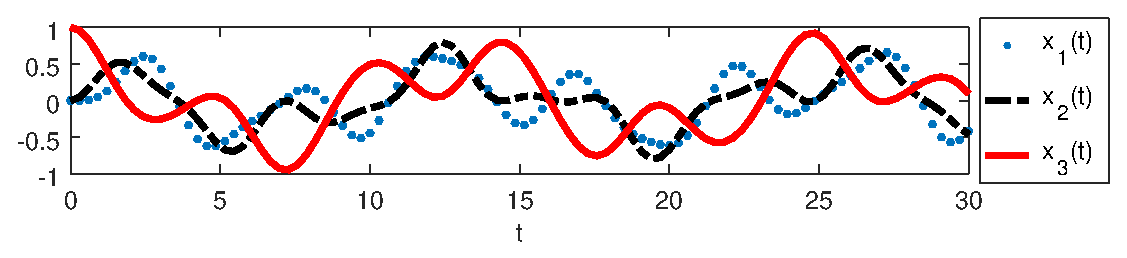
\includegraphics[width=0.99\textwidth]{chapters/differential-eq/mfiles/segundoorder/segundoroder1.eps}
         \caption{Resposta $\VECTOR{x}(t)$ do Exemplo \ref{ex:ddxPx:0}.}
         \label{fig:ex:ddxPx:0}
     \end{figure}
